\setauthor{Antonio Kuvac}

Die erste und auch längste Phase dieses Projekts war die Planung. 
In der Planungsphase wurden verschiedenste Kreativitätstechniken angewandt und Dokumente, die für die Planung unerlässlich sind, erstellt.

\section{Projektpartnermeetings}
\setauthor{Antonio Kuvac}

Der Grundstein für diese Arbeit waren die abgehaltenen Meetings mit dem Projektpartner dieses Projekts. Bei den ersten Meetings wurde definiert, was die App können muss und wie die App auszusehen hat
um Missverständnisse im voraus zu behandeln und um sich ein Bild darüber zu machen, welche Anforderungen das Projekt hat und welche Herausforderungen zu bewältigen sind. 
Mit diesen Meetings wurde der Projektpartner auch auf aktuellen Stand gehalten und auftretende Probleme und Anmerkungen, 
die bei der Arbeit am Projekt entstanden sind, wurden besprochen und abgehandelt.

\section{Use-Case Diagramm}
\setauthor{Antonio Kuvac}

Ein Use Case Diagramm oder auch Anwendungsfalldiagramm ist ein Diagramm von Anwendungsfällen und ihren Beziehungen zu ihrer Umgebung und zu anderen Anwendungsfällen. 
Damit beschreibt es, welche Funktionen und Dienste ein System für einen Anwender bereitstellt.
Mit einem Use Case Diagramm werden weder die Abläufe des Systems beschrieben, 
noch die Reihenfolge der Funktionen oder Dienste dargestellt. 
Ein Anwendungsfalldiagramm visualisiert lediglich die Zusammenhänge zwischen einer Menge von Use Cases und den involvierten Akteuren. Damit eignet es sich sehr gut zur Anforderungsanalyse, also zur Ermittlung oder Verfeinerung von Anforderungen.
\pagebreak
\subsection{Elemente im Use-Case Diagramm}

Folgende Elemente sind in einem Use-Case Diagramm üblicherweise enthalten:
\begin{itemize}
    \item System: Das System ist an sich kein logisches Modellelement, sondern grenzt den Kontext ab. Das System wird durch eine Box im Diagramm dargestellt, in dem das System seine Funktionen und Dienste zur Verfügung stellt.
    \item Akteur: Der Akteur befindet sich außerhalb des Systems. Er wird als Strichmännchen gezeichnet und kann eine konkrete Person aber auch ein abstraktes Element wie zum Beispiel ein Sensor sein. Wird ein Akteur definiert, muss dieser auch immer mit mindestens einem Use Case in Verbindung stehen.
    \item Anwendungsfall: Ein Anwendungsfall wird meistens als Ellipse visualisiert. Ein Diagramm kann mehrere Anwendungsfälle besitzen. Ist ein Use Case nur durch andere Anwendungsfälle ausführbar, wird er als abstrakt bezeichnet.
    \item Beziehungen: Zwischen Akteuren und Anwendungsfällen oder zwischen Anwendungsfällen selbst bestehen Beziehungen. Sie werden meistens als Linien oder Pfeile zwischen den jeweiligen Objekten eingezeichnet.
    \item Notizen: Mit Notizen lassen sich Informationen hinzufügen, um das Verständnis zu erhöhen. Sie werden mit einem Rechteck dargestellt, dessen obere rechte Ecke eingeknickt ist. Eine gestichelte Linie verbindet die Notiz mit dem zu erklärenden Element.
    
    \end{itemize}
    \pagebreak
    \subsection{Verwendung des Use-Case Diagramms in der Diplomarbeit}

    Das Use Case Diagramm wurde verwendet um Klarheit über die Funktionen und den Akteuren zu schaffen und für Vergewisserung zu sorgen, dass keine wichtigen Verbindungen vergessen wurden.
    Am Ende der Planungsphase angelangt sieht das Use-Case Diagramm wie folgt aus:

    \begin{figure}[H]
        \centering
        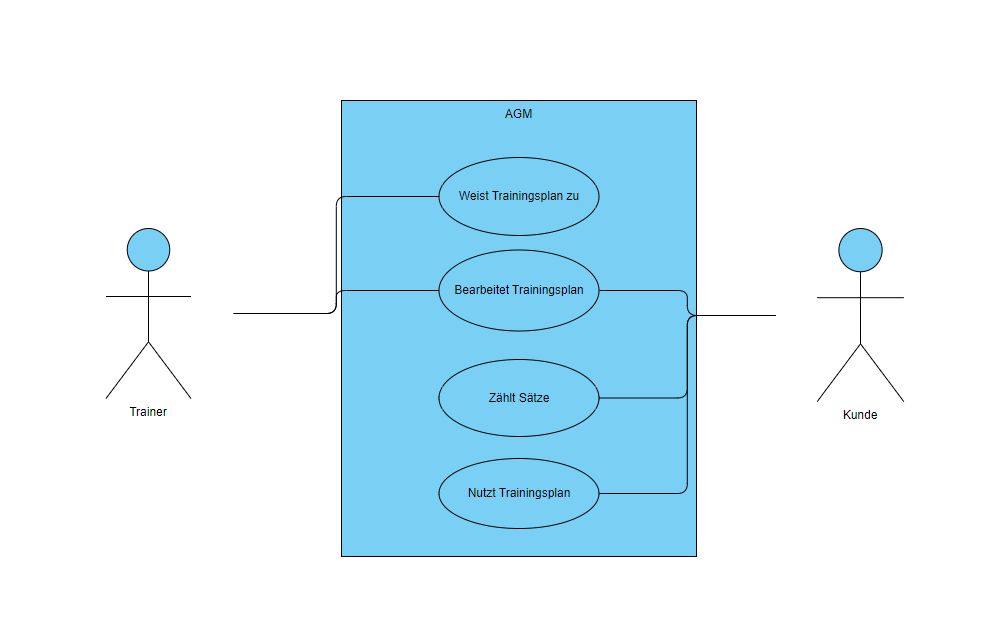
\includegraphics[scale=0.6]{pics/Use Case Diagramm.png}
        \caption{Use-Case Diagramm}
    \end{figure}


    \section{Entity Relationship Diagram - ERD}
    \setauthor{Antonio Kuvac}

    Ein ERD ist ein Diagramm der Beziehungen (Relationship) zwischen Entitäten (Entity) in einem Datenbankschema darstellt. 
    Es wird verwendet, um das Design einer Datenbank zu modellieren und darzustellen und wie Daten in der Datenbank organisiert und miteinander verbunden sind.

    \pagebreak

    \subsection{Komponenten eines ERDs}

    Üblicherweise bestehen ERD-Diagramme aus drei Hauptkomponenten, und zwar aus Entitäten, Attributen und Beziehungen.

    \begin{itemize}
        \item Entitäten: Eine Entität repräsentiert eine Klasse von Objekten, die bestimmte Eigenschaften oder Attribute gemeinsam haben. Ein Beispiel für eine Entität wäre zum Beispiel ein Kunde der als Attribute einen Namen und eine Wohnadresse hat. Entitäten werden meistens als Rechtecke dargestellt
        \item Attribute: Attribute sind die Eigenschaften, die die Entitäten beschreiben, wie beispielsweise der Name eines Kunden oder die Menge eines Produkts. Attribute werden meistens durch Ellipsen dargestellt können aber auch in der Entität selbst drinnen stehen.
        \item Beziehungen: Beziehungen beschreiben die Art und Weise, wie Entitäten miteinander in Verbindung stehen. 
        Man unterscheidet zwischen drei Arten von Beziehungen. Die erste ist One-to-One.  Diese Beziehung tritt auf, wenn jeder Datensatz in der ersten Tabelle nur einen entsprechenden Datensatz in der zweiten Tabelle hat und umgekehrt. Ein Beispiel dazu wäre eine Person und sein Reisepass, denn jede Person hat nur einen Reisepass und ein Reisepass gehört nur zu einer Person.
        Die zweite Art ist One-to-Many. Diese Beziehung tritt auf, wenn ein Datensatz in der ersten Tabelle mehrere Datensätze in der zweiten Tabelle hat. Ein Beispiel dafür ist eine Mutter die mehrere Kinder hat, aber jedes Kind hat nur eine leibliche Mutter.
        Die Letzte Art von Beziehung ist Many-to-Many.Diese Beziehung tritt auf, wenn ein Datensatz in der ersten Tabelle mehrere Datensätze in der zweiten Tabelle hat, aber auch umgekehrt. Ein Beispiel für diese Beziehung ist ein Student der mehrere Kurse hat und ein Kurs der mehrere Studenten hat.

        \end{itemize}

        \pagebreak

    \subsection{Verwendung des Entity Relationship Diagrams in der Diplomarbeit}

    Um eine funktionierende Datenbank für das Backend zu gewährleisten wurde in Zusammenarbeit mit den Mitgliedern vom Projekt AberGym  mithilfe eines ERDs eine Datenbankstruktur erstellt die sowohl für die Anforderungen von AberGym als auch für die Anforderungen von AberGymMobile angepasst.